\subsection{Постановка задачи}
3.5. Вычислить определенный интеграл $$F = \[ \int_{x_0}^{x_1} y \,dx \]$$, 
методами прямоугольников, трапеций, Симпсона с шагами $h_1, h_2$. Оценить погрешность вычислений, используя  Ме­тод Рунге-Ромберга: 

{\bfseries Вариант:} 19
    \begin{equation}
		y = x^2, 625-x^4; X_0 =0 , X_k =4, h_1 = 1.0, h_2 = 0.5
    \end{equation}
\pagebreak

\subsection{Результаты работы}
\begin{figure}[h!]
\centering
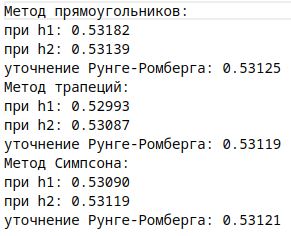
\includegraphics[width=.5\textwidth]{lab3.5}
\caption{Вывод в консоли}
\end{figure}


\subsection{Исходный код}
\lstinputlisting[title=\texttt{Lab3.5.cpp}]{../stud/saifullin/task3.5/Lab3.5.cpp}
\pagebreak

